\section{Discussion}

\marginpar{
\begin{figure}
  \begin{center}
  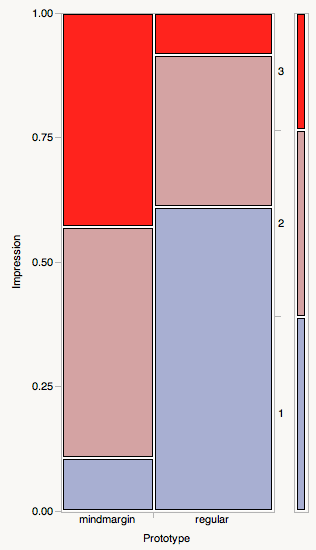
\includegraphics[width=\marginparwidth]{fitleastsqs_hypoth1.png}
  \caption{When using MindMargin, participants with prior exposure to the article reported less extreme stance.}
  \label{fig:leastsqs}
  \end{center}
\end{figure}
}


The lower SP values among MindMargin users reveal that participants with MindMargin who had prior exposure to the article reported less polarized views to reading the article for a second read or glance. 

However, there are limitations to our observations, as the results suggest that our trends are not yet statistically significant. This could likely result from using a between-subjects methodology. To address this in subsequent research, we plan to significantly increase the participant pool and to employ a within-subjects methodology, in which we query participants for their individual stance prior to their reading of the article and observe the deltas in SP values afterward. 

MindMargin users had a significantly more positive impression of the comments. Since all participants were exposed to identical comments, we conclude that MindMargin readers consider the comments more substantial and ultimately place greater trust and consideration into others' opinions.

In addition to our results, we would like to acknowledge some anecdotal evidence from a MindMargin user that suggests actions he/she took beyond the scope of reading and commenting article:``This article showed me a new perspective on TFA, which after doing research, I have realized I agree with.`` No written feedback suggesting actions outside the scope of the article was received from participants with the traditional commenting system. While there is insufficient evidence to conclude that MindMargin motivated the participant's pursuit of further research into the issue, it nevertheless indicates that this particular participant, exposed to the MindMargin interface, thought critically and independently about the issue discussed in the article.